\chapter{Luminosity measurement at CMS experiment}  %Title of the First Chapter

\ifpdf
    \graphicspath{{Chapter2/Figs/Raster/}{Chapter2/Figs/PDF/}{Chapter2/Figs/}}
\else
    \graphicspath{{Chapter2/Figs/Vector/}{Chapter2/Figs/}}
\fi

%\section{Luminosity measurement at CMS experiment}
%\label{sec:luminositycms}

%Luminosity measurement is a crucial aspect of particle physics experiments such as the Compact Muon Solenoid (CMS) experiment at the Large Hadron Collider (LHC). Luminosity refers to the rate at which particles collide within the detector, and accurate measurement of luminosity is essential for precise determination of particle collision rates and cross-sections. The CMS experiment uses several different devices to measure luminosity, including the Pixel Luminosity Telescope (PLT), Fast Beam Condition Monitor (BCM1F), Hadron forward (HF), Drift tubes (DT), radiation monitoring system for environment and safety (RAMSES) as shown in Fig.~\ref{fig:lumino_cms}. The DT luminometer covers the pseudorapidity range from 0 to 1.2, which is the central region of the CMS detector. The PCC luminometer covers the pseudorapidity range from 0 to 2.5, which covers the central and forward regions of the CMS detector. The HF luminometer covers the pseudorapidity range from 3 to 5, which is the most forward region of the CMS detector. The BCM1F luminometer covers the pseudorapidity range from 3.1 to 4.7, which is also in the forward region of the detector. The RAMSES luminometer covers the pseudorapidity range from 4 to 5, which is also in the forward region of the detector. The PLT luminometer covers the pseudorapidity range from 2.8 to 4.7, which is in the forward region of the CMS detector as shown in Fig.~\ref{fig:lumino_cms_pseudo}. In addition, the Pixel Cluster Counting (PCC) and zero counting method are a commonly used techniques for luminosity measurement at the CMS experiment.

%Luminosity measurement is a crucial aspect of particle physics experiments such as the Compact Muon Solenoid (CMS) at the Large Hadron Collider (LHC). Luminosity signifies the rate at which particles collide per unit area per second, making its precision measurement vital for the precise determination of particle collision rates and cross-sections.

The CMS experiment employs several devices to measure luminosity, each covering specific pseudorapidity ranges and regions within the CMS detector \cite{CMS-PAS-LUM-18-002}. The use of several luminometers as shown in Fig.~\ref{fig:lumino_cms} offers a multitude of advantages. Primarily, it ensures redundancy and acts as a backup for potential device failures, ensuring that data collection can proceed without interruption. Additionally, having multiple luminometers allows for cross-checking, providing greater consistency in results and allowing for more reliable data interpretation. These different devices enable better control over systematic uncertainties, as any discrepancies can be identified and adjusted for. Moreover, each device employs different method to measure luminosity, providing complementary information that enriches the overall understanding of particle interactions. Some luminometers recording low rates can be calibrated using others, enhancing their accuracy and utility. This holistic approach to luminosity measurement significantly improves the robustness and reliability of the data collected. In the central region, the Muon Drift Tubes (DT) luminometer is used covering a $\eta$ range from 0 to 1.2. The Pixel Cluster Counting (PCC) luminometer also operates in this region and extends into the forward region covering a range from 0 to 2.5. In the forward region, several devices are utilized. The Pixel Luminosity Telescope (PLT) covers the pseudorapidity range from 2.8 to 4.7. The Fast Beam Condition Monitor (BCM1F) functions in a range from 3.1 to 4.7. The Radiation Monitoring System for Environment and Safety (RAMSES) are located directly behind HF. The Hadron forward (HF) luminometer caters to the most forward region of the CMS detector \cite{Sirunyan:2759951}, functioning in the pseudorapidity range from 2.9 to 5.2 as shown in Fig.~\ref{fig:lumino_cms_pseudo}.

%In addition to these devices, two common techniques used for luminosity measurement at the CMS experiment are the Pixel Cluster Counting (PCC) and zero counting method. Please refer to Figures 1.1 and 1.2 for further visual information about these devices and their respective coverage within the CMS detector.

\section{Luminosity measurement methods}

%\subsubsection{Luminosity measurement devices at the CMS Experiment}

\begin{itemize}

%\item Pixel Luminosity Telescope (PLT) : The PLT consists of six planes of silicon pixel sensors, which are placed around the beam pipe, covering a total of 13.6 meters in length. Each sensor is divided into many small pixels, which are sensitive to charged particles passing through them. The sensors are positioned at a distance of about 2 mm from the beam center and measure the number of particles that pass through them. Silicon pixel sensors are divided into pixels of size 100 $\times$ 150 $\mu m^2$. The sensors have a thickness of 285 µm and are designed to operate at high radiation levels. PLT's luminosity measurement is to count the number of particles produced in the proton-proton collisions that pass through the silicon pixel sensors. The more particles that pass through the sensors, the higher the luminosity of the collisions. When a proton-proton collision occurs, it produces a shower of particles that pass through the sensors, creating a "hit" in each sensor. The PLT then uses the number of hits recorded by each sensor to determine the luminosity of the collisions.

\item Pixel Luminosity Telescope (PLT) : PLT is positioned 1.75 meters away from the interaction point, the PLT is an ensemble of 16 "telescopes." These are symmetrically distributed around the beam pipe at both extremities of the detector, with each telescope being composed of three individual silicon sensor planes. A defining feature of the PLT's functionality is the measurement of per-bunch instantaneous luminosity. This is accomplished by enumerating events in which all three sensor planes in a given telescope simultaneously register a hit. A specialized readout mechanism operating at the LHC's full bunch-crossing frequency of 40 MHz is employed to carry out this task. The PLT has provisions for reading out full pixel data, albeit at lower frequencies. This less frequent, yet detailed data readout serves multiple purposes. It is instrumental in determining calibrations, implementing corrections, and evaluating systematic uncertainties associated with both online and offline measurements. The PLT operates in what is called the "fast-OR" mode, which detects charged particles produced in a single bunch crossing of the proton beams. In this mode, the PLT triggers on any pixel in the detector that registers a signal above a certain threshold. This signal is called the "fast-OR signal" and indicates that a charged particle has passed through the detector. The PLT uses the information from all three detector planes to reconstruct the trajectories of the charged particles produced in the collisions. This is done by analyzing the signals from the individual pixels and using algorithms to determine the path of the particle through the detector.
  %The PLT consists of four layers of silicon pixel sensors arranged in a stack, with each layer containing over 8 million individual pixels. The first three layers are located very close to the interaction point where the proton beams collide, and the fourth layer is located further away. The innermost layer is located 2.9 cm from the interaction point. The second layer is located 3.9 cm from the interaction point. The third layer is located 4.9 cm from the interaction point. The outermost layer is located 10.2 cm from the interaction point \cite{Ayala:2861814}. The pixel sensors are designed to detect charged particles produced in the collisions as they pass through the detector layers. The PLT operates in what is called the "fast-OR" mode, which detects charged particles produced in a single bunch crossing of the proton beams. In this mode, the PLT triggers on any pixel in the detector that registers a signal above a certain threshold. This signal is called the "fast-OR signal" and indicates that a charged particle has passed through the detector. The PLT uses the information from all four detector planes to reconstruct the trajectories of the charged particles produced in the collisions. This is done by analyzing the signals from the individual pixels and using algorithms to determine the path of the particle through the detector.
  %To measure the luminosity of the collisions, the PLT counts the number of charged particles produced in each bunch crossing, and uses this information to calculate the rate of collisions. The luminosity is then calculated by dividing the collision rate by the cross-section of the proton-proton interactions.
  The PLT uses a specialized algorithm called the "triple coincidence" to identify charged particles that are produced in the collisions and to reject background noise. It requires a charged particle to be detected in all three planes, which corresponds to a "triple coincidence" detection. The rate of triple coincidences is proportional to the luminosity. This helps to reduce the contribution of background noise and improve the precision of the luminosity measurement \cite{Lujan:2017kvh}.

\item Fast Beam Conditions Monitor (BCM1F) : The BCM1F is specifically designed to detect the ionization produced by charged particles passing through its diamond sensors, and to convert this signal into a measurement of the beam intensity and luminosity. The BCM1F consists of 24 diamond sensors, each with an active area of 1 cm², arranged in six rings around the beam pipe. The diamond sensors are positioned very close to the CMS detector, just 10 cm away from the beam pipe. This allows the sensors to detect the charged particles produced by the proton-proton collisions. When charged particles pass through the diamond sensors, they ionize the carbon atoms in the diamond crystal, producing electrons and holes. The electrons and holes are then collected by metal electrodes embedded in the diamond, producing a voltage signal proportional to the ionization produced by the charged particles. The voltage signal is then amplified by fast electronics and converted into a digital signal, which is sent to the CMS data acquisition system for further analysis. To measure the luminosity, the BCM1F counts the number of charged particles passing through each diamond sensor per unit time. The signal from each sensor is integrated over a short time interval (usually 25 ns), corresponding to the time it takes for a single proton bunch to pass through the sensors. The integrated signal is then converted into a measure of the instantaneous luminosity, which is proportional to the product of the number of charged particles per bunch and the collision frequency.

  %The number of charged particles per bunch is determined by calibrating the BCM1F with data from other detectors in the CMS experiment, such as the silicon pixel detector and the pixel luminosity telescope. These detectors are used to measure the total number of charged particles produced by the proton-proton collisions, which is then used to calibrate the BCM1F \cite{CMS-DP-2013-003}.

%\item Fast Beam Conditions Monitor (BCM1F) : The BCM1F measures the luminosity by detecting the particles that are produced in the proton-proton collisions and scattered at very small angles from the beam direction. These particles, called "forward protons," travel along the beamline and can be detected by the BCM1F. The BCM1F consists of two arrays of scintillating fibers, placed symmetrically around the beam pipe, at a distance of about 20 cm from the beam center. The fibers are sensitive to charged particles passing through them, and their signals are used to measure the position and intensity of the forward protons. The forward protons that are detected by the BCM1F travel along the beamline and reach the end of the detector at different times, depending on their energy and direction. The time-of-flight (TOF) of each proton is measured by using the difference in arrival times between the two arrays of scintillating fibers. The BCM1F measures the luminosity of the proton-proton collisions by counting the number of forward protons that pass through the detector and by measuring their time-of-flight. 

%\item Beam Halo Monitor (BHM):  The Beam Halo Monitor (BHM) is a device used in particle accelerators to measure the halo of particles that surround the main beam. The halo is a region of low-density particles that surrounds the main beam and can cause damage to accelerator components or experimental detectors. The BHM is designed to detect these halo particles and measure their flux. The BHM consists of two arrays of scintillating fibers, placed on either side of the beam pipe. The fibers are arranged in a grid pattern and are sensitive to the ionization produced by charged particles passing through them. When a halo particle passes through a fiber, it produces scintillation light, which is detected by photomultiplier tubes at the ends of the fibers. The signal from the photomultiplier tubes is then processed by electronics to provide a measurement of the halo flux. To measure the luminosity, the BHM uses a technique called "optical theorem," which relates the total scattering cross-section of the halo particles to the luminosity of the beam. The scattering cross-section is the probability that a halo particle will scatter off a proton in the main beam, and is proportional to the luminosity of the beam. The BHM measures the total scattering cross-section by counting the number of halo particles passing through the scintillating fibers and calculating the fraction of particles that scatter off the main beam. This fraction is then used to calculate the luminosity of the beam. One advantage of the BHM is that it can detect halo particles with energies as low as a few keV, making it sensitive to a wide range of halo particles. It is also a non-destructive technique, which means that it does not affect the main beam or experimental detectors.

%\item Beam Halo Monitor (BHM): The BHM measures the luminosity by detecting the particles that are produced in the proton-proton collisions and scattered at large angles from the beam direction. These particles, called "beam halo," can interact with the BHM sensors and produce signals that are proportional to the luminosity. The BHM consists of a set of sensors that are placed around the beam pipe, at a distance of about 1.6 meters from the beam center. The sensors are sensitive to charged particles passing through them, and their signals are used to measure the position and intensity of the beam halo. The signals from the BHM sensors are processed to extract the information about the beam halo. The signals are first amplified and shaped, and then digitized and recorded. The recorded data are then used to reconstruct the position and intensity of the beam halo. The BHM measures the luminosity of the proton-proton collisions by detecting the beam halo particles that interact with the BHM sensors and produce signals. 

\item Hadron Forward Calorimeter: The Hadron Forward (HF) Calorimeter is a critical component of the CMS experiment. It is a subdetector that measures the energy, position and arrival time of particles produced during proton-proton collisions. The HF Calorimeter is designed specifically to measure hadron particles, which are particles made up of quarks and gluons, in the forward region (i.e., close to the beamline) of the CMS detector. The HF Calorimeter is located at the very front and back of the CMS detector, at a distance of about 11.2 meters from the interaction point. This placement allows it to cover a pseudorapidity range of 2.9 to 5.2, which is important for measuring particles produced at small angles relative to the beamline. The HF Calorimeter is a sampling calorimeter, which means it consists of alternating layers of active and passive materials. The active material, in this case, is scintillating quartz fibers, which emit light when they interact with charged particles. The passive material is steel absorber plates, which serve to initiate hadron showers, causing the incident hadron to interact and create secondary particles. As these secondary particles pass through the scintillating fibers, they produce light, which is collected by photodetectors and converted into an electrical signal proportional to the particle's energy. Two separate algorithm are used for luminosity measurement in the HF Calorimeter, HFOC and HFET based on the Zero Counting (ZC) method and the Missing Transverse Energy (MET) methods respectively \cite{CMS-PAS-LUM-15-001}. 

%The Zero Counting method is a threshold-based approach for estimating the luminosity. In this method, the total number of inelastic collisions, which produce new particles, is counted by measuring the energy deposited in the HF Calorimeter. To separate inelastic collisions from background noise and other processes, a threshold on the energy deposition is applied. During data-taking, the HF Calorimeter measures the energy deposited in each bunch crossing (when two bunches of protons pass through each other in the LHC). When the energy deposition in both HF Calorimeter sides (HF+ and HF-) is below a certain threshold, it is considered a "zero count" event, which means no inelastic collision has occurred. The number of zero count events is subtracted from the total number of bunch crossings, giving the number of inelastic collisions. The luminosity can then be calculated by dividing the number of inelastic collisions by the integrated time and the inelastic cross-section. The ZC method has the advantage of being robust against pile-up (simultaneous multiple proton-proton collisions) since it relies on counting the events where no energy is deposited. However, it may be affected by detector noise and other background processes that can lead to a non-zero energy deposition.
The zero counting method is used by particle colliders to measure the luminosity. In this method, the luminosity is estimated by counting the number of events with zero particles detected in a specific region of the detector. The basic idea behind the zero counting method is that the probability of having zero particles detected in a given region of the detector is proportional to the probability of having no collisions in that region. This probability can be related to the luminosity of the collisions through the following equation:

\begin{equation}
L = \frac{-ln(N/N_0)}{\sigma_{vis}}
\end{equation}

where L is the luminosity, N is the number of events with zero particles detected in the region of interest, $N_0$ is the total number of events, $\sigma_{vis}$ is the visible cross-section. One advantage is that it is a simple and robust method that does not require sophisticated detectors or calibration procedures. However, it can be affected by background events, such as cosmic rays or beam-gas interactions, which can produce zero particles in the region of interest and increase the uncertainty in the luminosity measurement. \\
The Missing Energy method is an alternative approach for luminosity measurement in the HF Calorimeter. This method relies on measuring the total transverse energy (Et) deposited in the calorimeter and comparing it with the expected average transverse energy for inelastic collisions. The idea behind the MET method is that the total transverse energy should be conserved in a collision event. Inelastic collisions are expected to produce a certain amount of transverse energy on average, which can be estimated from simulations and theoretical calculations. The missing energy in an event is defined as the difference between the expected average transverse energy and the measured transverse energy in the HF Calorimeter. For each bunch crossing, the missing energy is calculated, and a distribution of missing energy values is obtained. This distribution is then fitted to a functional form, which includes a term for the inelastic collisions and terms for various background processes (e.g., detector noise, beam-gas interactions). The fit allows extracting the number of inelastic collisions, which can then be used to calculate the luminosity. The MET method is sensitive to the energy scale calibration of the detector and the modeling of background processes. However, it provides an independent and complementary measurement to the ZC method, which helps to reduce systematic uncertainties in the luminosity determination \cite{Sirunyan:2759951}.

%\item Hadron Forward Calorimeter: The HF sub-detector measures the luminosity by detecting the neutral particles produced in the proton-proton collisions that interact with the hadron forward calorimeter. These particles include neutrons, photons, and neutral hadrons, and they are produced in the forward region of the detector at a large pseudorapidity, which means they are produced at small angles with respect to the beam axis. The HF sub-detector consists of two arrays of steel absorbers, each followed by radiation-hard quartz fibers that detect the Cherenkov light produced when particles pass through them. The two arrays are placed symmetrically on either side of the beam pipe at about 11 meters from the interaction point. The signals produced by the quartz fibers are collected and digitized to produce time and energy measurements of the particles that pass through the Hadron Forward Calorimeter. The HF sub-detector measures the luminosity of the proton-proton collisions by counting the neutral particles that interact with the Hadron Forward Calorimeter and using this information to calculate the luminosity. 

%\subsubsection{Luminosity measurement techniques at the CMS Experiment}

\item Muon drift tubes: The DT system is part of the CMS muon system, %which also includes the Resistive Plate Chambers (RPCs) and the Cathode Strip Chambers (CSCs).
  Drift Tubes (DTs) in the CMS experiment are designed to accurately measure the trajectory and momentum of muons produced in proton-proton collisions at the LHC.
  %The DT system is located in the barrel region of the CMS detector, covering the pseudorapidity range of $|\eta| < 1.2$.
  The DT system consist of rectangular drift cells filled with a gas mixture, typically of argon and carbon dioxide. The use of DT muon rates for luminosity measurement is based on the idea that the rate of single muon production is proportional to the instantaneous luminosity. Single muons comes from decay of inclusive, Z, W, top and jets.
%The DT system in the CMS detector is used for muon detection and precise position measurement. Drift Tubes are essentially gas-filled detectors. When muons pass through these tubes, they ionize the gas. The resulting ions and electrons drift under the influence of an electric field to anode wires located in the center of the tubes, producing a signal. By measuring the drift time, one can infer the position of the muon's trajectory.
To use the DT muon rates as a luminometer, one would need to count the rate of detected muons as a function of the delivered luminosity. However, the DT muon rate luminometer is not independently calibrated during the Van der Meer (vdM) scan due to low measured rate. It is cross calibrated with PCC or HF.
  
  %Each drift cell contains a thin anode wire held at a high voltage relative to the cell walls, which act as the cathode. When a charged particle like a muon passes through the gas-filled cell, it ionizes the gas molecules, producing free electrons and positively charged ions. These free electrons drift towards the anode wire under the influence of the electric field, while the positive ions drift towards the cathode. The drift time of electrons to the anode wire is measured, and by knowing the drift velocity in the gas mixture, the distance between the ionizing particle's trajectory and the anode wire can be determined. Combining the information from multiple drift cells, the trajectory of the muon can be reconstructed with high precision. It is not a primary method for luminosity measurement, as the system is specifically designed for muon detection and momentum measurement. However, one could potentially use the muon rates detected by the DT system for an indirect luminosity measurement. This would involve correlating the rate of muons detected in specific processes, such as those from W and Z boson decays, with the underlying luminosity. By measuring the rate of these processes and comparing them to the known production cross-sections, the luminosity could be inferred. This approach would require careful control of various experimental factors, such as the efficiency and acceptance of the DT system, the precise determination of the production cross-sections, and corrections for pile-up and background processes. It is important to note that this would not be a primary luminosity measurement technique, but it could provide a complementary cross-check to the main methods used in the CMS experiment \cite{Chatrchyan:2013sba}.

\item Pixel Cluster Counting (PCC): The pixel detector in the CMS experiment is made up of multiple layers of silicon sensors arranged in a cylindrical shape around the beam pipe. When charged particles from the collisions pass through the silicon sensors, they create electric charge that is read out as a signal. The signals from adjacent sensors are combined to form clusters, which represent the position of the particle track in the detector. The total number of clusters detected over a certain period of time is used to estimate the luminosity. The PCC provides a precise measurement of the luminosity and is particularly useful when the collision rate is high \cite{CMS-PAS-LUM-13-001}.

\end{itemize}

\begin{figure}[!htp]
\centering
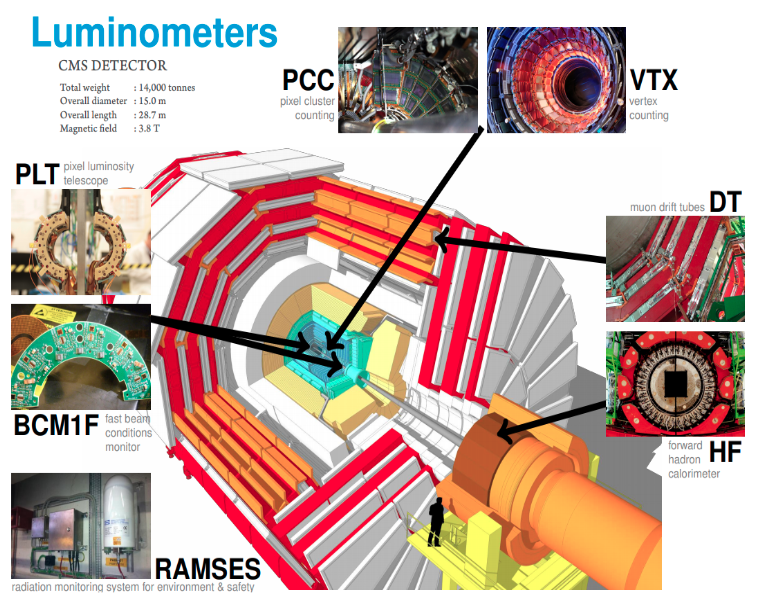
\includegraphics[width=0.9\textwidth]{ashish_thesis/luminometer_cms.png}
\caption[CMS Luminometers]{%
   CMS detector with all of the luminosity measurement devices showing PLT, BCM1F, HF, DT, PCC and RAMSES \cite{meyer2021luminosity}. 
}
\label{fig:lumino_cms}
\end{figure}


\begin{figure}[!htp]
\centering
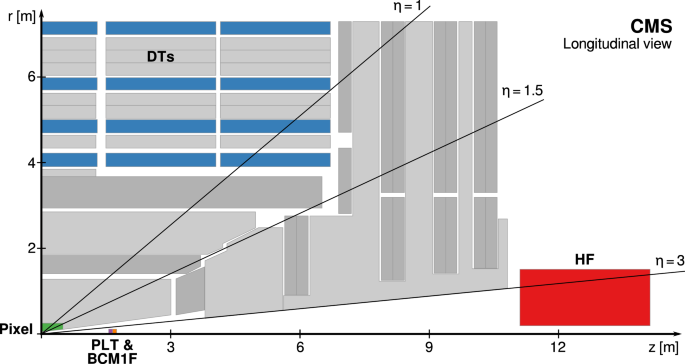
\includegraphics[width=0.9\textwidth]{ashish_thesis/luminometer_cms_pseudo.png}
\caption[CMS luminometers Location]{%
    Cross section of the CMS detector in the r-z plane showing all Run 2 luminometer PLT, BCM1F, DTs, and HF location. The two RAMSES monitors used as a luminometer in Run 2 are located directly behind HF \cite{Sirunyan:2759951}. 
}
\label{fig:lumino_cms_pseudo}
\end{figure}

%\newpage
\section{Pixel detector}

The pixel detector is one of the subdetectors of the CMS experiment that is closest to the interaction point where the proton beams collide. It consists of four barrel layers (L1-L4) at radii of 29, 68, 109 and 160 mm and three forward disks (D1-D3) on each end at distances of 291, 396, and 516 mm of pixel sensors from the center of the detector as shown in Fig.~\ref{fig:phaseI_upgrade}. It is built from 1856 silicon sensor modules, 1184 modules in the barrel layers (BPIX) and 672 modules for the forward disks (FPIX) \cite{Adam:2748381}. Modules for barrel layers and forward disks are shown in Fig.~\ref{fig:pixelmodule}. Table~\ref{tab:modpix} shows the number of modules in each pixel layer and disk. The modules in BPIX L1 are designed to handle high particle densities and radiation levels. Each module in this layer consists of a matrix of 4160 pixels, arranged in 160 rows and 26 columns. The pixel size in BPIX L1 is approximately 100x150 µm², which allows for high-resolution position measurements of charged particles. The modules in BPIX L2-4 layers are designed to withstand lower radiation levels compared to BPIX L1. Each module in BPIX L2-4 consists of a matrix of 66560 pixels, arranged in 260 rows and 256 columns. The pixel size in BPIX L2-4 is also approximately 100x150 µm². The FPIX modules are also designed to handle high particle densities and radiation levels. Each module in the FPIX consists of a matrix of 16128 pixels, arranged in 160 rows and 101 columns with same pixel size as layer pixels.
%It provide high-precision position measurements of the charged particles produced in the collisions. These position measurements are used to reconstruct the trajectories of the particles and to identify the particles themselves.
The pixel detector has a high position resolution, with a spatial resolution of 4.8  microns in the transverse direction and 7.99 microns in the longitudinal direction. The pixel detector also has a high time resolution, with a readout time of 25 nanoseconds. The pixel detector is capable of detecting charged particles with a wide range of energies, from a few hundred MeV to several TeV. The pixel detector is able to operate at very high particle fluxes, with a hit rate of up to $100 MHz/cm^2$. To achieve this high rate capability, the pixel detector uses fast readout electronics.
%which can read out the signals from the pixels in a few microseconds.
The pixel detector is also designed to operate at a high radiation level, with a dose of up to $5 \times 10^{14} neutrons/cm^2$ expected over the lifetime of the detector. To mitigate the effects of radiation damage, the pixel detector uses sensors made of high-purity silicon and a cooling system that keeps the detector at a temperature of -20°C. The pixel detector is  used as a primary luminometer. The luminosity measurement is based on counting the number of pixel clusters produced in the detector by the proton-proton collisions.  However, there are several challenges to accurately measure the luminosity with the pixel detector. One challange is the multiple proton-proton collisions per bunch crossing (pileup). Another challenge is the non-linearity of the pixel detector response, which can lead to inaccuracies in the luminosity measurement. Therefore, the motivation of this research work is to develop and test more precise techniques for measuring the luminosity with the pixel detector.

\begin{figure}[!htp]
\centering
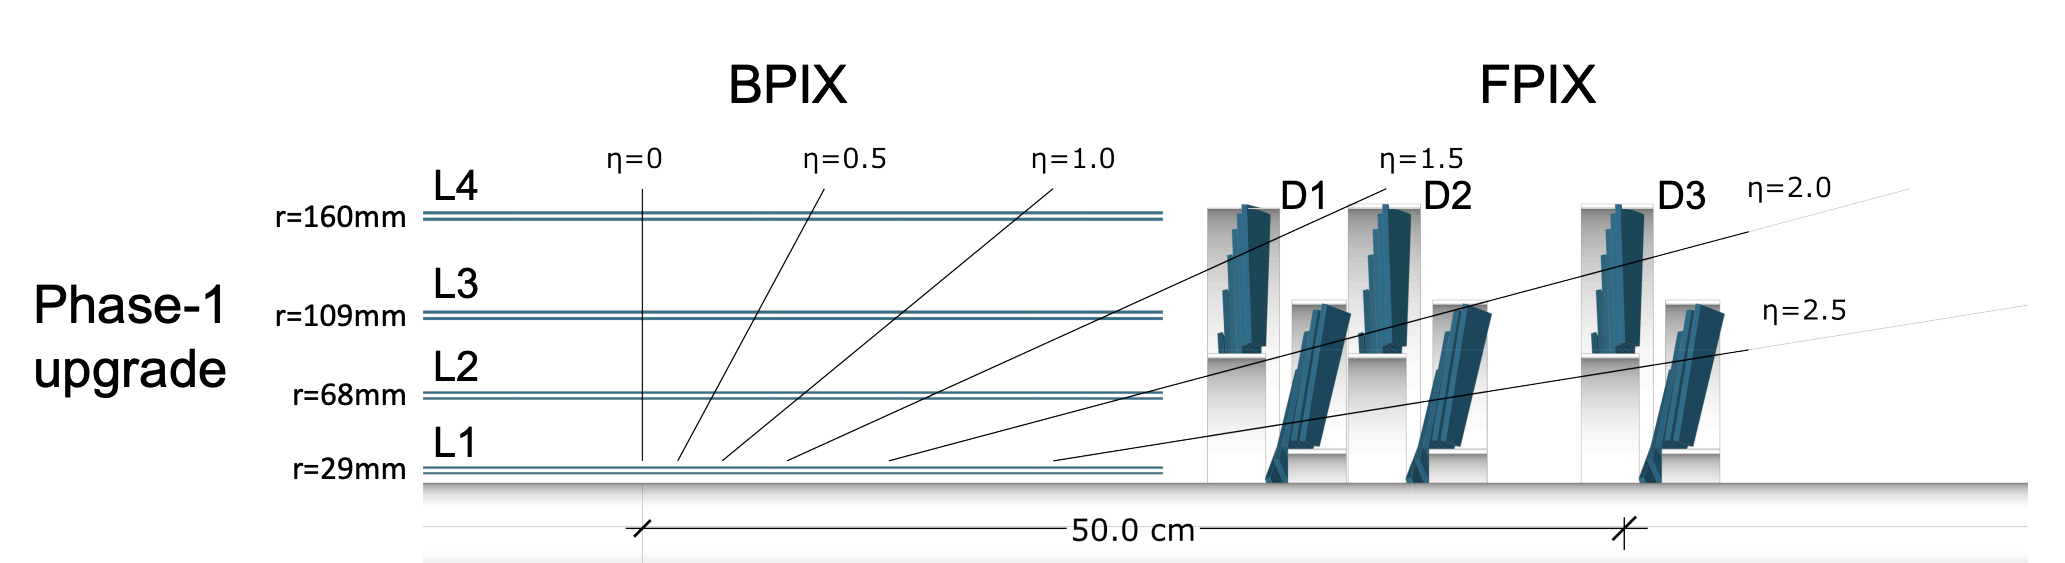
\includegraphics[width=1\textwidth]{ashish_thesis/phaseI_upgrade_pixel_detector.png}
\caption[Pixel Detector Layout]{%
   Layout of the CMS Phase-1 upgraded pixel detector in longitudinal view \cite{Adam:2748381}. 
}
\label{fig:phaseI_upgrade}
\end{figure}


\begin{figure}[!htp]
\centering
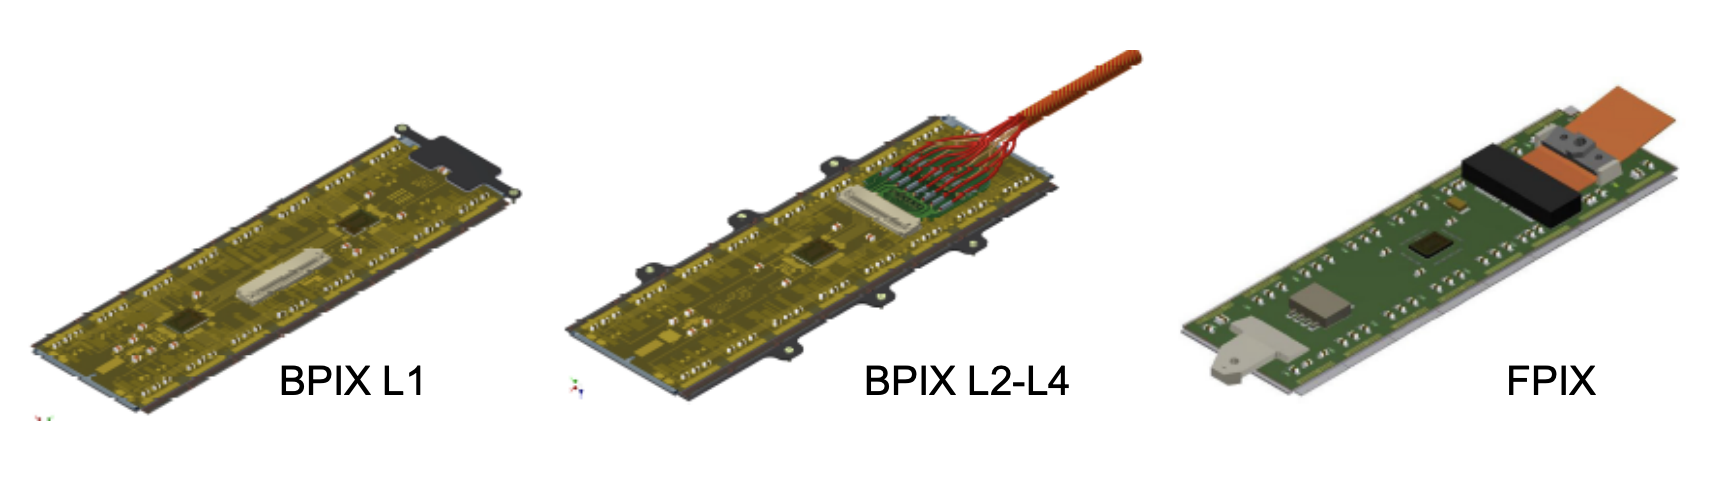
\includegraphics[width=1\textwidth]{ashish_thesis/silicon_pixel_module.png}
\caption[Pixel Module Design]{%
   Pixel detector modules for BPIX L1 (left), BPIX L2-4 (middle), and
the FPIX detector (right) \cite{Adam:2748381}. 
}
\label{fig:pixelmodule}
\end{figure}


\begin{table}
  \begin{center}
    \caption[Number of modules in pixel layers and disks]{Number of pixel detector modules in each layer and disk.}
    \begin{tabular}{ccccc}  
    \textbf{Layer/Disk}   & \textbf{\# modules} \\ \hline
     L1      &    96        \\  
       L2    &     224   \\ 
        L3   &       352 \\ 
         L4   &       512 \\ 
         D1 inner ring & 88     \\ 
         D1 outer ring &   136    \\ 
         D2 inner ring &      88 \\ 
         D2 outer ring &   136   \\ 
          D3 inner ring&     88  \\ 
         D3 outer ring &    136  \\ 
      \end{tabular}
    %\caption[Number of modules in pixel layers and disks]{Number of pixel detector modules in each layer and disk.}
    \label{tab:modpix}
  \end{center}
\end{table}


\section{Pixel cluster counting (PCC) method}

The Pixel Cluster Counting (PCC) method is one of the main luminosity measurement technique used at the CMS experiment. The PCC method is based on counting the number of pixel clusters produced by the collisions in the CMS pixel detector, which is a high-resolution silicon detector located close to the collision point. The pixel detector is made up of more than 124 million pixels. The detector is designed to detect charged particles produced in the collisions, and the pixel clusters are formed when several neighboring pixels are hit by a single particle. The PCC method is based on the assumption that the number of pixel clusters produced is proportional to the number of collisions, and therefore to the luminosity. The proportionality constant is called the pixel detector visible cross section, and it can be determined with a calibration method described in section 3.1. The PCC method is implemented in two stages: the online and offline stages. In the online stage, the pixel clusters are counted in real time by the CMS data acquisition system, which uses a custom-designed ASIC chip to process the pixel detector signals. %The online luminosity measurement is therefore available within seconds of the collisions, and it is used to monitor the stability of the detector and to provide feedback to the LHC operators.
In the offline stage, the raw data from the pixel detector is analyzed using dedicated software to determine the pixel clusters and to calculate the luminosity. The offline luminosity measurement is more accurate than the online measurement, as it takes into account various corrections and calibrations that are not possible in real time. %The offline luminosity measurement is also used to determine the absolute luminosity scale, which is obtained from beam parameters.
There are several steps involved in the PCC method for measuring luminosity like data acquisition, pixel cluster reconstruction, pixel cluster counting as described below.

\begin{itemize}

\item Pixel detector data acquisition is the process of collecting and digitizing the signals from the silicon pixel detectors in the CMS experiment. When a particle passes through the silicon pixel detector, it creates a small amount of charge in the pixel sensor. The charge is collected by the electrodes in the pixel sensor and converted into a voltage signal. The voltage signal is then digitized using an analog-to-digital converter (ADC) to create a digital signal. The ADC measures the voltage at regular intervals, called sampling intervals, and assigns a digital value to each voltage measurement. The digital signal is then stored in a buffer in the front-end electronics of the pixel detector. The buffer is a small amount of memory that temporarily holds the data before it is transmitted to the data acquisition system. The data acquisition system continuously monitors the data from the pixel detectors to detect interesting events. When an event of interest is detected, a trigger signal is sent to the front-end electronics of the pixel detector to read out the data from the buffer. The readout electronics in the pixel detector then transmit the data to the data acquisition system using high-speed optical fibers. The data is sent in packets, called data frames, which contain information about the event, such as the time of the event, the position of the particle, and the amount of charge deposited in the pixel sensor. %The data acquisition system processes the data frames to reconstruct the particle tracks and identify the types of particles that passed through the pixel detector. The data is then stored in a format that can be used for further analysis.

\item Pixel cluster reconstruction is the process of identifying groups of adjacent pixels that have been fired by a single particle passing through the detector. The first step in the pixel cluster reconstruction process is to identify individual pixel hits in the data frames obtained from the pixel detector data acquisition system. A pixel hit is a small region of the pixel detector where charge has been deposited by a particle. The next step is to identify "seed" pixels, which are individual pixels with a high signal-to-noise ratio. A seed pixel is defined as a pixel hit with a signal above a certain threshold, which is typically set at a few times the noise level of the pixel detector. Once seed pixels have been identified, the next step is to build pixel clusters around each seed pixel. This is done by adding adjacent pixels with a signal above a lower threshold, called the cluster threshold. The cluster threshold is typically set at a level that minimizes the number of fake clusters while maximizing the efficiency of cluster finding. After pixel clusters have been built, the next step is to split or merge clusters as needed. This is done to remove fake clusters caused by noise or overlapping particles, and to merge clusters that are split due to inefficiencies in the cluster building process. Once the pixel clusters have been identified and merged/split as necessary, they are parameterized by their position and energy. The position of the cluster is determined by the center of gravity of the pixels in the cluster, and the energy is determined by summing the signal of all the pixels in the cluster. Finally, a set of selection criteria are applied to the pixel clusters to remove any remaining fake clusters and select only those clusters that are likely to be from real particle interactions. These selection criteria typically include requirements on the size, shape, and energy of the clusters.

\item The number of pixel clusters is counted over a fixed time intervals, known as lumi section. One lumi section is 23.36 seconds time interval. In the pixel cluster counting process, events of interest are selected from the large dataset obtained from the CMS experiment. This is typically done using zero bias triggers that select events that are coming from filled bunch crossing.
  %Once the events of interest have been selected, reconstruction the pixel clusters in each event is done using the steps described in the previous bullet point.
  %This involves identifying individual pixel hits, identifying seed pixels, building pixel clusters around each seed pixel, and parameterizing the clusters.
  After the pixel clusters have been reconstructed in each event, the next step is to count the number of clusters in each event. This can be done using simple counting algorithms that count the number of clusters above a certain energy threshold. %or more sophisticated algorithms that use machine learning techniques to identify and count clusters.
  The number of pixel clusters in each event is affected by various sources of background noise. %such as electronic noise and cosmic ray background.
  To accurately measure the number of signal clusters in each event, these background sources must be subtracted from the total cluster count.
 %This can be done using techniques such as sideband subtraction or template fitting. %Finally, to obtain an accurate measurement of the number of particles that passed through the pixel detector, the cluster counts must be corrected for the inefficiencies in the cluster reconstruction process. This can be done using simulation or other techniques to estimate the efficiency of the cluster finding algorithm as a function of the particle energy, position, and type.

%\item The number of pixel clusters is calibrated to account for various factors that affect the luminosity measurement, such as the efficiency of the pixel detector and the beam intensity. The calibration step is an important part of the PCC (Pixel Cluster Counting) method for measuring luminosity at the CMS experiment. The purpose of calibration is to account for various factors that can affect the measurement of the number of pixel clusters, which is directly proportional to the number of collisions that occurred during a given time interval. These factors include the efficiency of the pixel detector and the beam intensity. The efficiency of the pixel detector refers to the probability that a charged particle passing through the detector will create a signal in one or more pixels. The efficiency of the detector can vary with time, and it can also depend on the energy and angle of the charged particle. To account for the detector efficiency, calibration factors are applied to the number of pixel clusters that are counted. These calibration factors are determined by comparing the number of pixel clusters measured by the detector to the number of collisions predicted by other detectors or simulations. The beam intensity refers to the number of protons circulating in the LHC at any given time. The beam intensity can vary over time and can affect the measurement of the collision rate. To account for the beam intensity, the number of pixel clusters is normalized by the instantaneous luminosity, which is a measure of the collision rate at the interaction point. The instantaneous luminosity is determined by other detectors or by theoretical calculations. After applying the calibration factors, the number of pixel clusters is converted to the number of collisions that occurred during the given time interval. This number is then used along with other parameters such as the frequency at which the LHC is operating and the size of the interaction region to calculate the luminosity of the collision using the formula $L = \frac{N_{cl}  f_{rev}} {\sigma_{vis}} $. The resulting luminosity measurement provides valuable information about the collision rate and the physics processes occurring at the CMS experiment.

\item The number of pixel clusters is used to calculate the luminosity using the following formula:

\begin{equation}
 L_b = \frac{N_{cl} f_{rev} } {\sigma_{vis}}   
\end{equation}

where $L_b$ is the bunch luminosity, $N_{cl}$ is the number of clusters per bunch crossing, $f_{rev}$ is the revolution frequency of the LHC, and $\sigma_{vis}$ is the visible cross section of the pixel detector obtained from calibration.

\end{itemize}


The PCC method has several advantages over the other luminosity measurement methods used by the CMS experiment. The PCC method is based on the pixel detector, which has a high spatial resolution and can accurately measure the position and energy of charged particles. Another advantage is its high precision and stability, as it is based on a well-understood physical process and has a small systematic uncertainty. %Another advantage is its independence from the beam conditions, as the pixel detector is insensitive to the beam halo and the beam-gas interactions.
The PCC method is also robust against pile-up, which is the presence of multiple proton-proton interactions in a single bunch crossing, as it can distinguish between pixel clusters produced by different collisions. %The PCC method is based on the pixel detector, which has a high spatial resolution and can accurately measure the position and energy of charged particles.
This allows for precise measurements of the luminosity, even when the particle collision rate is high. The pixel detector has a high detection efficiency, meaning that it can detect a large fraction of the particles produced in the collisions. The pixel detector's high granularity enables precise detection of individual particles. %The pixel cluster counting method is relatively insensitive to pileup, allowing accurate luminosity measurements even when pileup is high,
It has a wide dynamic range, capable of measuring luminosities from low to high due to the large number of pixels.


\begin{comment}
  
Advantages of the PCC method are described below,


\begin{itemize}

\item High precision: The pixel detector has a high granularity and can detect individual particles with high precision. %This allows for a precise measurement of the luminosity, with uncertainties typically below 2\%.

\item High efficiency: The pixel detector has a high detection efficiency, meaning that it can detect a large fraction of the particles produced in the collisions. %This allows for a high signal-to-noise ratio and a low level of background noise, resulting in a more accurate measurement of the luminosity.

\item Long-term stability: The pixel detector has a high level of stability over long periods of time, which is important for accurate luminosity measurements over extended periods of data-taking.

%\item Fast and real-time: The pixel cluster counting method can provide luminosity measurements in real-time, allowing researchers to quickly analyze the data and make adjustments to the experiment as needed. This is particularly important for experiments that need to optimize their data-taking strategies based on the luminosity measurements.

\item Low sensitivity to pileup: Pileup refers to the number of additional collisions that occur within the same bunch crossing as the primary collision being studied. The pixel cluster counting method is relatively insensitive to pileup, meaning that it can still provide accurate luminosity measurements even when pileup is high. Thus, PCC is a linear luminometer.

\item Wide dynamic range: The pixel cluster counting method has a wide dynamic range, meaning that it can measure luminosities over a wide range of values, from low to high because of large number of pixels.



%This is important for experiments that need to measure luminosities over different energy ranges.

%\item Insensitivity to beam conditions: The pixel cluster counting method is relatively insensitive to beam conditions such as beam intensity and beam size. This makes it a reliable technique for luminosity measurement, even when the beam conditions vary.

%\item Independent of beam crossing angle: The pixel cluster counting method is independent of the beam crossing angle, which is the angle at which the beams intersect. This makes it easier to compare results obtained under different beam crossing angles.

%\item Independence from trigger systems: The PCC method operates independently of the CMS experiment's trigger systems, which means it is not affected by any biases or inefficiencies that might be present in the trigger.

\end{itemize}

\end{comment}

%However, the PCC method also has some limitations and challenges. One limitation is its sensitivity to the pixel detector efficiency and the noise level, as the cluster formation probability depends on the number of hit pixels and their signal-to-noise ratio. The PCC method also requires a precise knowledge of the pixel cluster cross section, which can be affected by various factors such as the beam spot size, the beam divergence, and the pile-up conditions. The PCC method is also affected by various sources of background, such as cosmic rays, machine-induced noise, and photon conversions, which can mimic pixel clusters produced by collisions. To mitigate these limitations and challenges, the CMS employs several techniques and strategies in the PCC method. One technique is the use of pixel clustering algorithms that are optimized for different beam conditions and pile-up levels, and that incorporate various quality criteria to reject noisy and fake clusters. Another technique is the use of dedicated calibration measurements using known luminosity sources, such as Van der Meer scans and beam-gas events, which provide a precise determination of the pixel cluster cross section and its variations as a function of the beam conditions. The CMS also employs various data-driven and simulation-based methods to estimate the background contributions and their uncertainties, and to correct for their effects on the luminosity measurement.

The PCC method has been extensively tested and validated by the CMS during the LHC Run 1 and Run 2, which corresponded to proton-proton collisions at center-of-mass energies of 7-8 TeV and 13 TeV, respectively. The PCC method has achieved a relative luminosity precision of about 1.5 \%, which is well within the design goals of the CMS \cite{CMS-PAS-LUM-18-002}. In the future, the PCC method will continue to be a key component of the CMS luminosity measurement strategy, as it provides a precise and robust measurement of the luminosity ratio between different datasets and periods. The PCC method will also benefit from the upgrades and improvements planned for the CMS pixel detector and the LHC, which will increase the luminosity and the collision rate, and will challenge the performance and the calibration of the PCC method. The CMS is planning to install a new pixel detector for the High-Luminosity LHC (HL-LHC) era, which will feature smaller pixel sizes, faster readout electronics, and radiation-hard materials. The CMS is also planning to develop new techniques and algorithms for the PCC method, such as machine learning methods, deep neural networks, and real-time analysis tools.

%The Pixel Cluster Counting (PCC) method is a powerful and reliable technique for measuring the luminosity of proton-proton collisions at the CMS detector at the LHC. The PCC method is based on the counting of pixel clusters produced by the collisions in the CMS pixel detector, and it provides a precise and stable measurement of the relative luminosity between different datasets and periods. The PCC method has several advantages, such as its high precision, stability, and independence from the beam conditions, and it has several limitations and challenges, such as its sensitivity to the pixel detector efficiency and the noise level, and its dependence on the pixel cluster cross-section and the background contributions. The PCC method has been extensively tested and validated by the CMS, and it will continue to play a crucial role in the future physics program of the CMS and the LHC.

%Pixel Cluster Counting (PCC) is a method for measuring the luminosity of particle collisions in high-energy physics experiments, such as those conducted at the Large Hadron Collider (LHC). The PCC method is based on counting the number of clusters of charged particles produced in the collision that are detected by the pixel detector of the experiment.

%Measuring the luminosity of particle collisions is an essential part of high-energy physics experiments. Luminosity is a measure of the rate at which particles are colliding and is directly related to the number of events observed in the experiment. The luminosity measurement is critical for understanding rare physics processes, such as the production of new particles or the measurement of the properties of known particles.

%Several techniques are used to measure luminosity in particle physics experiments, including the use of scintillators, Cherenkov detectors, and other radiation detectors. However, the most commonly used technique is the measurement of the rate of particles produced in the collision.

%The PCC method is based on counting the number of clusters of charged particles produced in the collision that are detected by the pixel detector of the experiment. The pixel detector is a high-resolution detector that is designed to provide precise measurements of the position and energy of charged particles.

%In the PCC method, the charged particles produced in the collision pass through the pixel detector, where they create clusters of pixels that are read out by the detector electronics. The number of clusters produced in each collision is proportional to the luminosity of the collision.

%In conclusion, the PCC method is a powerful technique for measuring the luminosity of particle collisions in high-energy physics experiments. The PCC method is based on counting the number of clusters of charged particles produced in the collision that are detected by the pixel detector of the experiment. The PCC method has several advantages over other luminosity measurement techniques, including its high spatial resolution, insensitivity to background radiation, insensitivity to the energy of the charged particles, and insensitivity to the material used in the detector. These advantages make the PCC method a valuable tool for understanding rare physics processes in particle physics experiments.

%Pixel cluster counting is the process of counting the number of pixel clusters that are reconstructed from the data acquired by the silicon pixel detectors during a given time interval, known as an LHC orbit. An orbit is the time it takes for the LHC to complete one revolution.

%The pixel detectors record the energy deposited by particles passing through them, and the data from the detectors is acquired by the CMS data acquisition system. The acquired data is then processed to reconstruct pixel clusters. A pixel cluster is a group of adjacent pixels that have been fired by a single particle passing through the detector. Pixel clusters are reconstructed using algorithms that take into account the shape and size of the charge deposited by the particles in the pixels.

%Once the pixel clusters are reconstructed, they are counted for a given time interval, typically the duration of one LHC orbit, which is about 89 microseconds. The number of pixel clusters is directly proportional to the number of collisions that occurred during that time interval. Therefore, counting the number of pixel clusters provides a way to measure the collision rate, which is an important input for calculating the luminosity of the collision.

%However, it is important to note that not all pixel clusters correspond to actual collisions. Some pixel clusters may be produced by background events, such as cosmic rays, that are not relevant for measuring the collision rate. Therefore, it is necessary to calibrate the number of pixel clusters to account for various factors that affect the luminosity measurement, such as the efficiency of the pixel detector and the beam intensity, before using it to calculate the luminosity.

%\section{Previous studies on PCC luminosity measurement}

The PCC of various layers and disks, normalized to the total PCC, as a function of lumi section can provide crucial insights into the detector's performance and stability over time and under different conditions \cite{CMS-PAS-LUM-15-001}\cite{CMS-PAS-LUM-16-001}. A lumi section is a unit of data-taking time in the LHC, typically lasting about 23.36 seconds, during which the beam conditions are assumed to be stable. The luminosity delivered during each of these lumi sections can vary, leading to different levels of activity in the detector.

When these ratios are plotted against lumi sections, several key aspects can be studied:

\begin{itemize}
\item Detector Stability: Stable ratios across lumi sections suggest that the detector is functioning consistently and reliably under varying luminosity conditions. Abrupt spikes or drops could be indicative of potential problems such as radiation damage, electronic noise, or other instabilities in the detector.

\item Long-Term Performance: By tracking these ratios over multiple lumi sections, one can monitor the long-term performance of the detector. This approach allows for the detection of gradual changes or trends, which could suggest a slow degradation of the detector components.

\item Layer/Disk-Specific Analysis: This type of plot can reveal layer or disk-specific issues. For instance, if one layer's PCC ratio deviates significantly from the norm in high lumi sections, it might suggest that this layer is particularly sensitive to low luminosity or is underperforming.

%\item Operational Adjustments: Observations from these plots can guide operational adjustments. If the PCC ratios for certain layers or disks consistently deviate under specific luminosity conditions, adjustments could be made in the detector operation to account for these variations.
\end{itemize}

\begin{comment}
  
The stability plots of the pixel detector for Run2018A, Run2018B and Run2018C are shown in Fig.~\ref{fig:RunA_PCC_ratios}, Fig.~\ref{fig:RunB_PCC_ratios}, Fig.~\ref{fig:RunC_PCC_ratios} respectively where the PCC ratios are not stable for some layers and disks with time. These PCC ratios as a function of luminosity sections, where each section represents about 23.36 seconds of data collection, allows physicists to conduct a nuanced evaluation of the pixel detector's performance and stability, identify potential issues, and make necessary operational modifications to ensure the detector's efficiency. 


\begin{figure}[!htp]
\centering
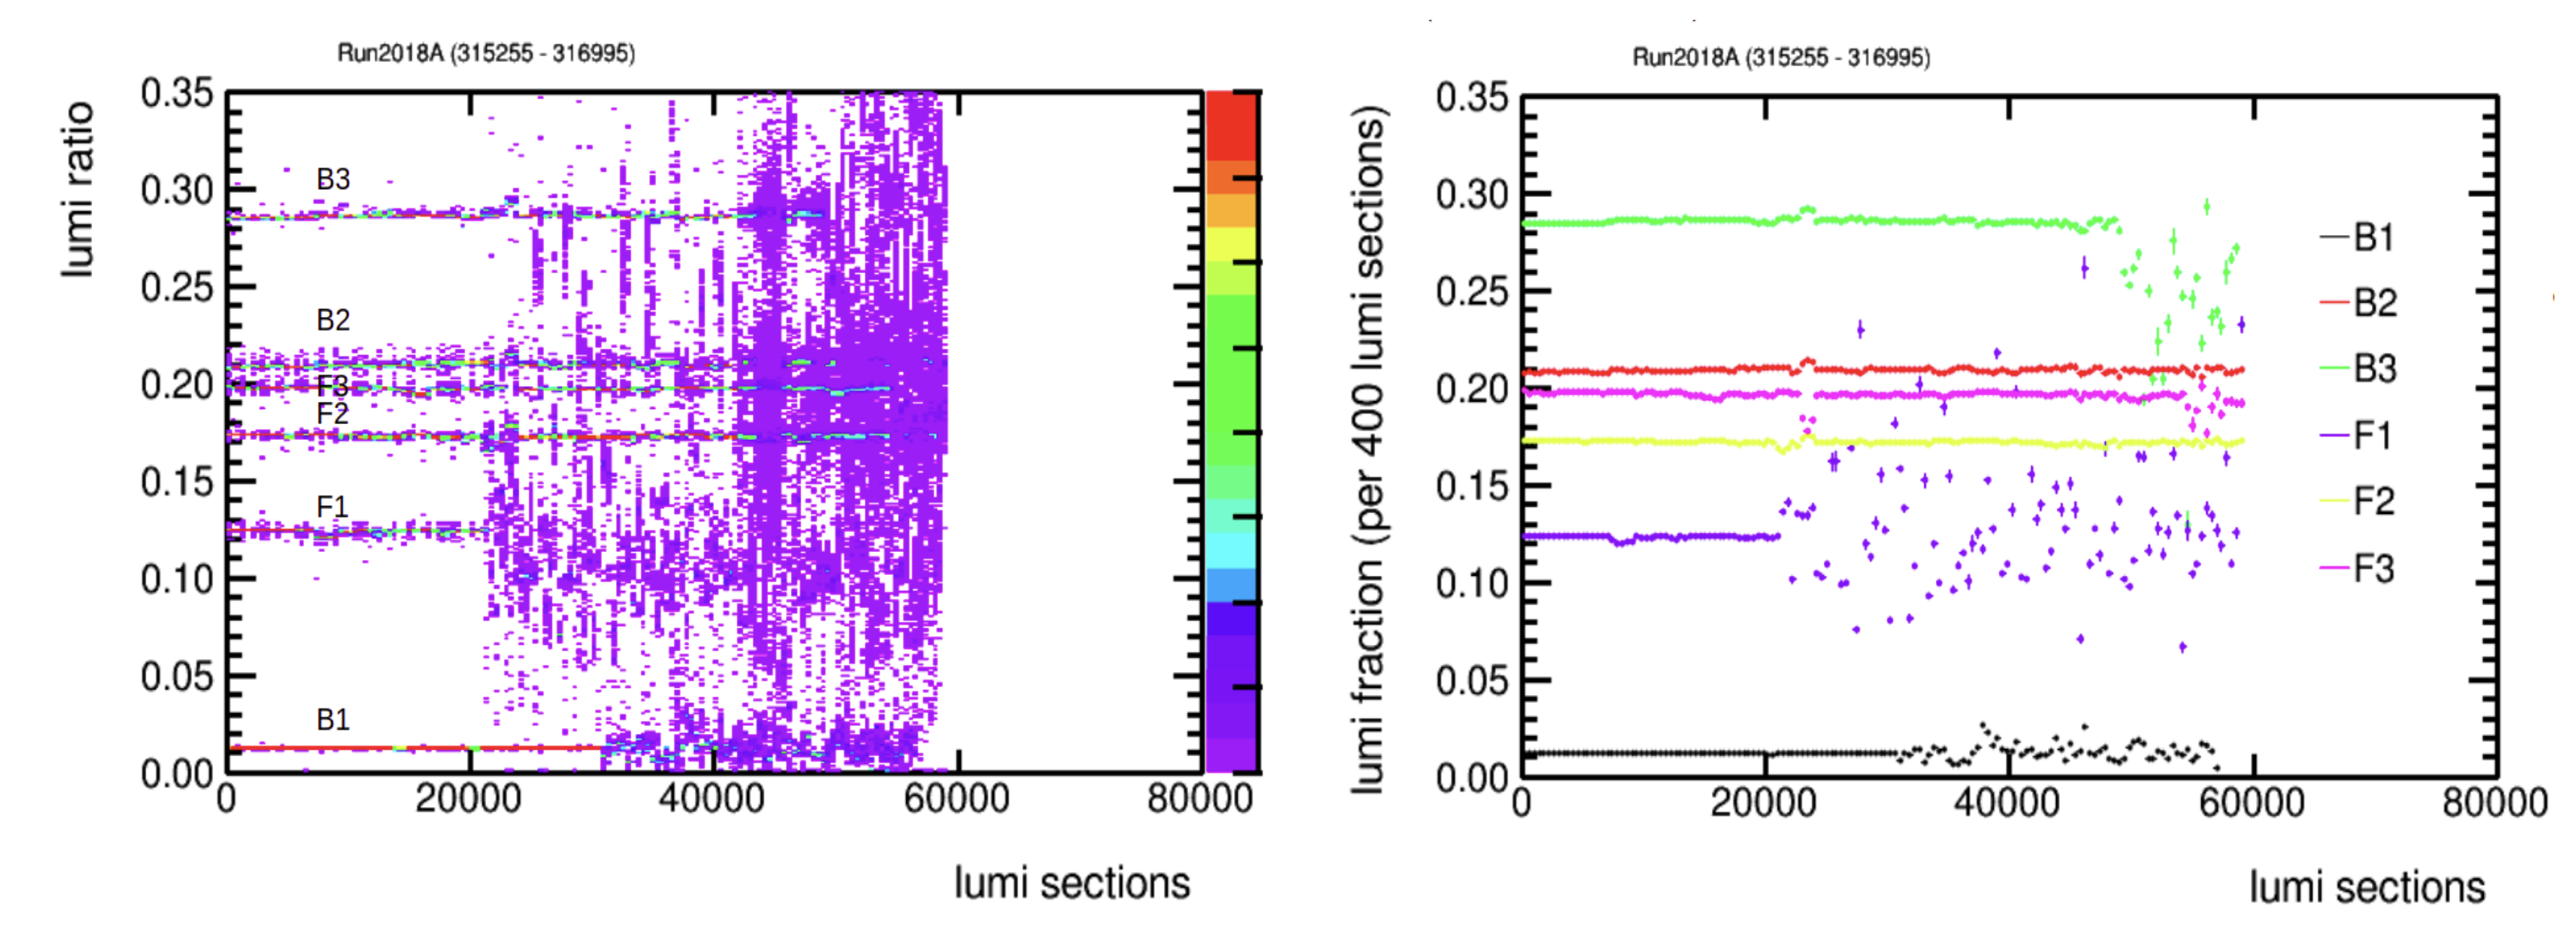
\includegraphics[width=1\textwidth]{ashish_thesis/Run2018A_old.png}
\caption[PCC ratios for period 2018A]{%
Left: Luminosity ratios for various sub detectors L2, L3, L4, D1, D2, D3 of pixel detector as a function of lumi section for Run2018A. Right: X Profile of luminosity ratios vs lumi section graph for various sub detectors L2, L3, L4, D1, D2, D3 of pixel detector showing luminosity fraction as a function of lumi section for Run2018A.

}
\label{fig:RunA_PCC_ratios}
\end{figure}


\begin{figure}[!htp]
\centering
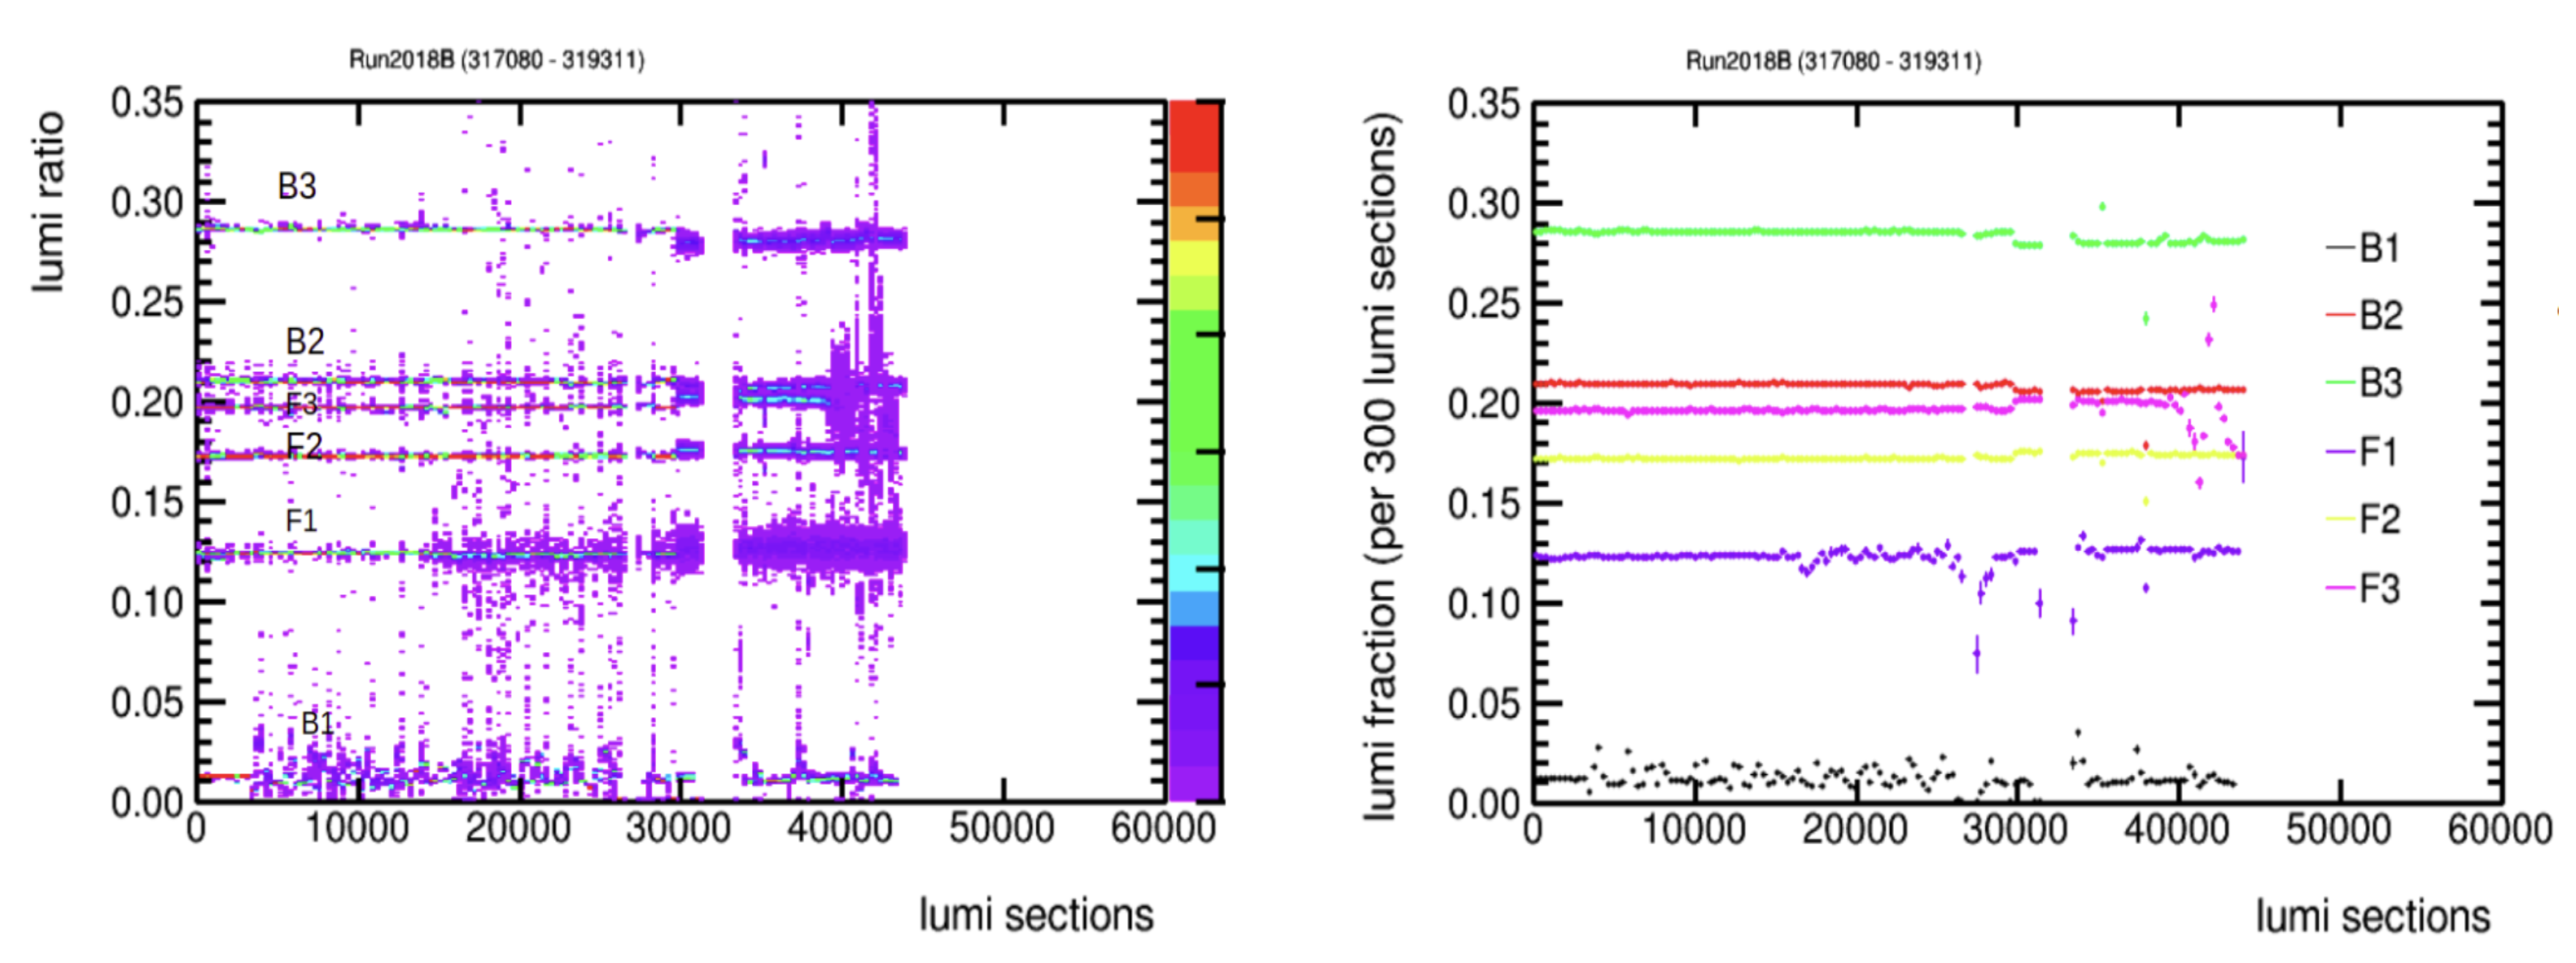
\includegraphics[width=1\textwidth]{ashish_thesis/Run2018B_old.png}
\caption[PCC ratios for period 2018B]{%
Left: Luminosity ratios for various sub detectors L2, L3, L4, D1, D2, D3 of pixel detector as a function of lumi section for Run2018B. Right: X Profile of luminosity ratios vs lumi section graph for various sub detectors L2, L3, L4, D1, D2, D3 of pixel detector showing luminosity fraction as a function of lumi section for Run2018B.
}
\label{fig:RunB_PCC_ratios}
\end{figure}


\begin{figure}[!htp]
\centering
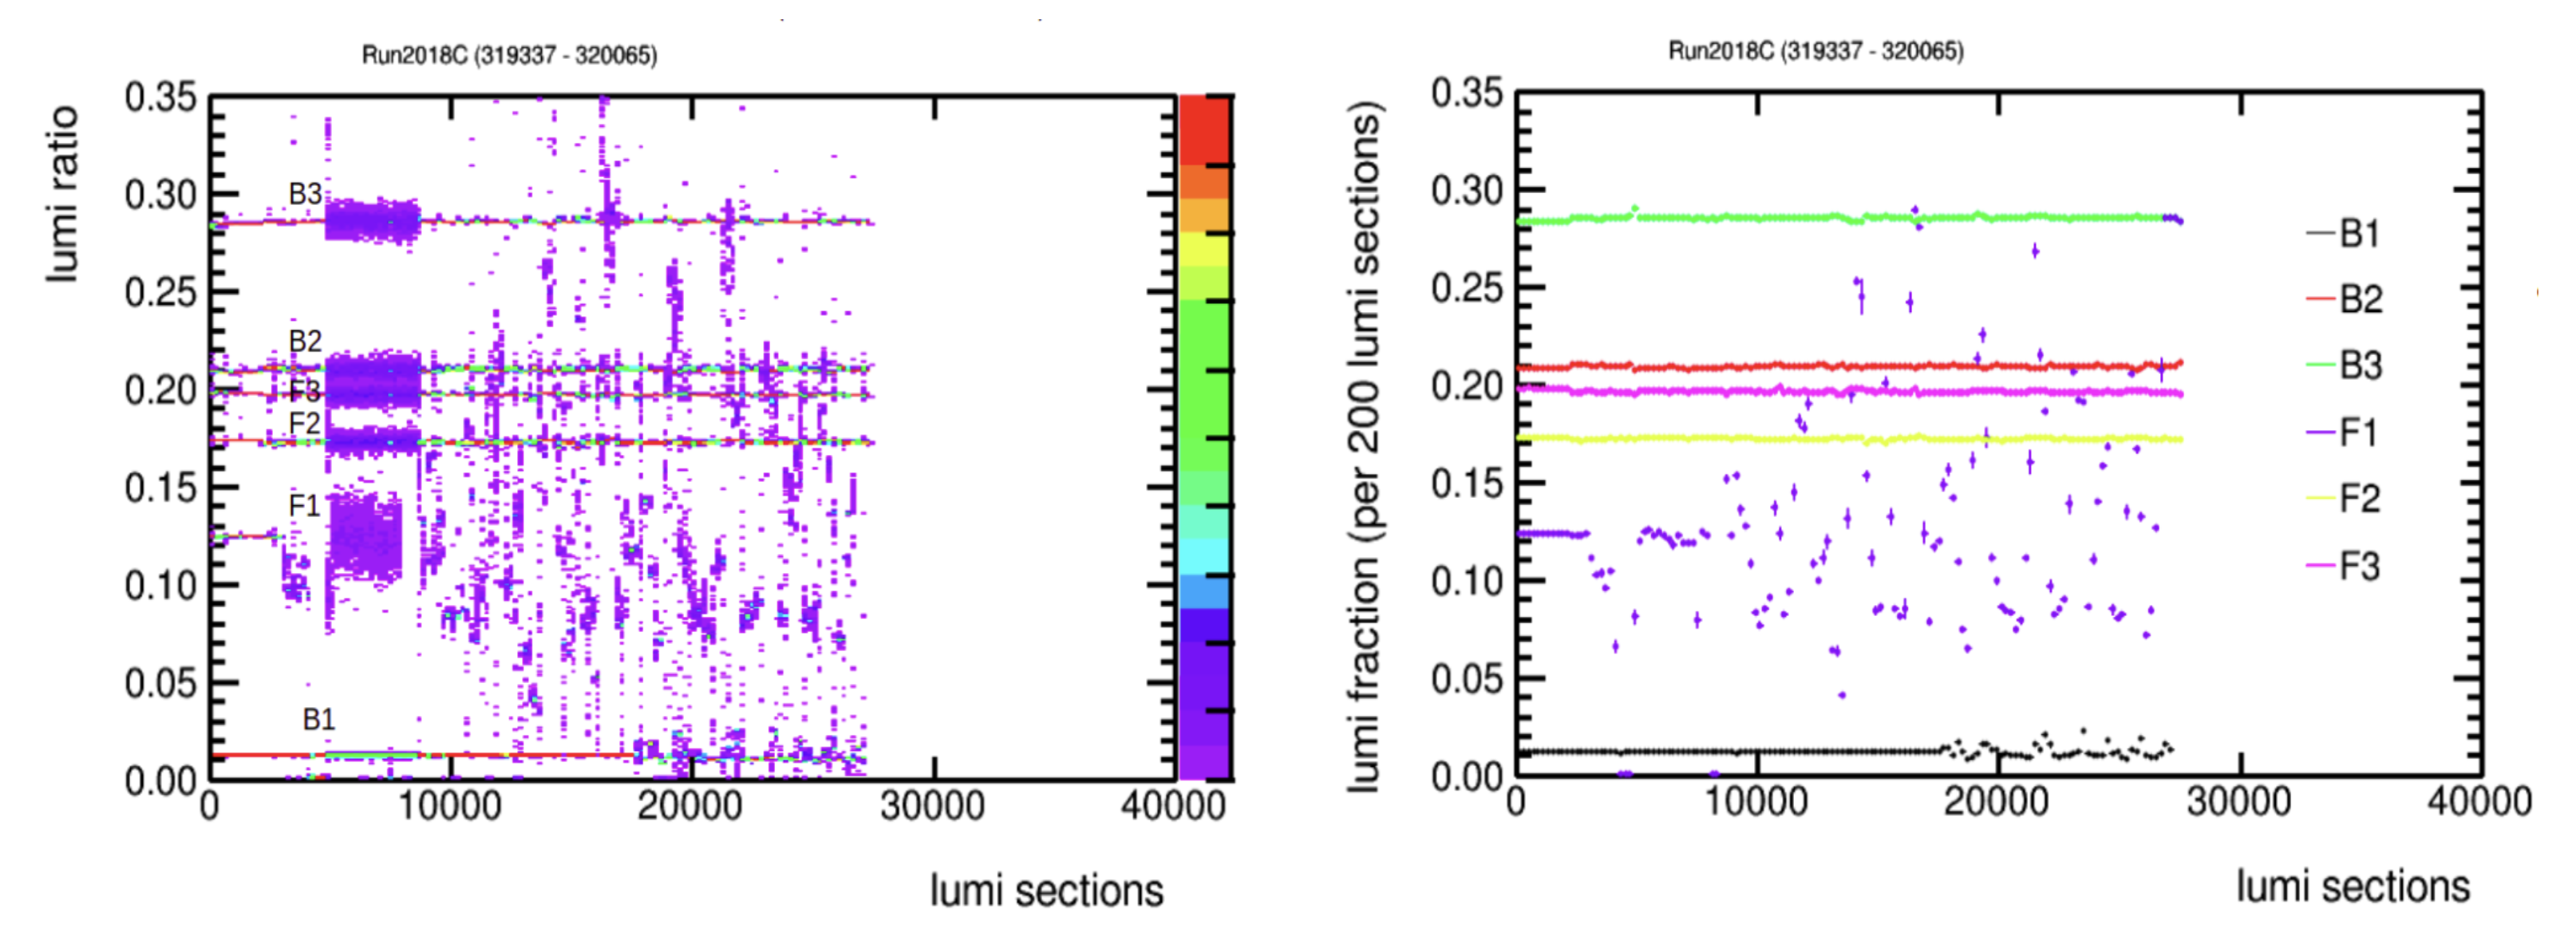
\includegraphics[width=1\textwidth]{ashish_thesis/Run2018C_old.png}
\caption[PCC ratios for period 2018C]{%
Left: Luminosity ratios for various sub detectors L2, L3, L4, D1, D2, D3 of pixel detector as a function of lumi section for Run2018C. Right: X Profile of luminosity ratios vs lumi section graph for various sub detectors L2, L3, L4, D1, D2, D3 of pixel detector showing luminosity fraction as a function of lumi section for Run2018C.
}
\label{fig:RunC_PCC_ratios}
\end{figure}

\end{comment}
